% Chapter 9

\chapter{Web Design Development} % Main chapter title

\label{Chapter 9} % For referencing the chapter elsewhere, use \ref{Chapter1} 

%----------------------------------------------------------------------------------------

This chapter aims to explain what choice were made and why from the web development point of view. It is interesting to analyse which are the particular requirements of this software and what solutions were chosen to satisfy them. 

\section{Requirements}

From the Web Development's point of view the first step to do is to identify what are the most important goal to achieve. They are uncorrelated but not conflict with the requirements already analysed related with the Human Machine Interaction's point of view. Following there are some observations:

\begin{enumerate}

% 1
\item
The first thing that it is important to guarantee is a strong division between front end and back end. This is because both part are important, but the way in which they work are very independent, and they can evolve in different ways.
As explained in the previous chapters the front-end, so the way in which the information is presented to the user is a particularly sensitive issue that needed a special attention and a deep analysis related to the interaction; The back-end is also important because needs to work on particular topics related to the communication with ROOT Framework, the security, the persistence of data. An important observation is that the front-end changes in the time, according to the new features and in reaction of the observations of the users, but the back-end changes faster. The challenge of the front-end is the needs to remain more stable and be re-usable when the logic behind, the back-end change. For example: almost twice a month the algorithms of the existing analysis of gAn change, and also new analysis are added (sometimes some old ones are removed). The output of the back-end changes rapidly, but almost always the front-end, that is flexible can manage automatically the situation showing the results to the users in an organized way. Also the drivers able to trigger the changes are different: the users for the front-end, the scientific progress of the experiments for the back-end. If these parts are completely (almost completely) independent it is surely all more simple. In principles it is also possible a complete substitution of the back-end: both with a different program able to implement analysis of data of the AEgIS experiment or with a completely different program able to work with runs, to give outputs formatted in text and images, and to be configured by an xml file.

%2
\item
Another quite important point to keep in mind is that this application will be maintained and probably modified by people that aren't specialized Web Developer. So it is important to maintain the code as simple as possible and to "hide" the complexity where a complex structure is unavoidable. For example, the functions able to read and write on files, to extract histogram from vectors, to apply "regular expression" to verify the format of a file can be packed into functions able to be simply called without expect expertise from the programmer.   

%3
\item
The logical separation between client and server implies that a way to communicate is needed. A simple communication based on Post and Get is quite effective, but a more structured communication based on exchange of complex object seems to be more re-usable, and simpler to maintain and modify. From this point of view Json language give a standard well known solution, simple, efficient, and effective to solve this issue  

%4
\item
The program of data analysis (gAn) need to be configured. Some of these configurations are accessible by the user, some aren't, but in both cases it is important to give a structured way to persist the configuration of the application. The first idea is to use a simple text file to achieve this goal, but with the growth of the file a more formal solution becomes preferable. Xml is a good solution, because it is a diffused standard and there are a lot of API and libraries able to help to write and read in an easy way.  

%5
\item
A simple but precise way to evaluate the formatting of a string or a group of strings is needed to ensure in every moment that the program is working with the correct value. For example, it is important to ensure that if the user is inserting a run number the entered value is effectively a decimal number: in other case the front-end can advise the user of the error. This first example is related to an inadvertent error, but it is important to consider also other situations when, for security reason, immediately before save a number in a file, or immediately before insert a number as a variable in a bash script the application needs to ensure that the value is compatible (so, has the same format) of the expected one. This is a prudential approach, but we must consider the this application is thought to work on a Intra-net, not, on the internet, so the occurrence of an attack is not so immediate. There are some solution considered to avoid problems and formatting objects correctly, the two effectively used are regular expressions to certify if a string respect some limits, and some standardized functions provided by Php to check if in a string there are dangerous commands.
 
%6
All the software must work easily with the Root Framework, so communicate with it using APIs or others way to interact with gAn. This is not always simply, because Root provides some APIs to communicate with languages used in web developing but there is a big lack of documentation. Often, in absence of documentation for some needed functionalities the best way to work was check directly the open source code of the APIs to understand the functionalities gave by them.

\end{enumerate}

\section{Why a web solution?}

Before start to work with this project using web development some other solution was evaluated:

\begin{enumerate}

% 1
\item 
The first solution considered was simply work with the commands of a common linux terminal. This is the solution implemented for gAn. This solution is surely powerful and effective, because gives the maximum control on the possible commands, allows pipelines, gives an immediate feedback in every moment (these features of the linux terminal are often ignored). However this is not the best possible available solution, because it presupposes a perfect understanding of the behavior of the program, and a very good memory to remember all the commands and all the possible analyzes. 
This solution is no longer used for the final application itself, but it is still very useful to debug the application in case of errors.   

% 2
\item
Another analysed solution was the creation of a stand alone application, with an advanced graphical interface, able to perform analyses on a common laptop or on the computers of the AEgIS control room. This solution is able to use all the advantages of the application of the human machine interaction science, but it is quite limited: in a hypothetical situation with this solution applied it would be very difficult give to all the users the same version of the application (that is changing continuously). So in that case a system able to check automatically the application for updates every "x" days would be necessary, and the total amount of complexity would be quite high. Other problems of these solution are that it would be able to work only with the LAN of the AEgIS Control Room to access the data that are stored on dedicated hard disks, and the computational power of a common laptop would have some problem to analyse data in a reasonable time (the data at the moment are some terabytes, but in the future this amount will probably growth rapidly).

%3
\item
Probably the better possible solution (the adopted one) is the web application. So with simply a web browser also a low quality laptop can access information, and both the data and the application are always at the last version (the application change quite rapidly, but actually new data are added every some hundreds of seconds every days when the machine is working.. so only a centralized application can meet the need to react to the continuous modification of the situation).
In this way the user doesn't need to install nothing, and this is an advantage because the practice shows that the installation process of gAn is not so linear and shows often configuration problems (the behavior of gAn is linked to the version of Root Framework installed on the machine, the different versions are not perfectly compatible). Another advantage of this solution is that in this way only the server needs to manage the problem to recover the data (at their most recent version) and to store them in an intelligent way. Furthermore the computational power of the server is probably more suitable to execute the requested analysis. It is important to reason about the possible request of parallel execution from more users at the same time, but considering the number of the total user of this application, that is around at maximum a few tens, the charge on the server to satisfy the multiple requests is not so high.    

\end{enumerate}
 
\section{MVC}

The application of the Model View Controller pattern is usually a good idea in Web Development, specially in an application that needs to be rapidly modified and needs a special attention to the maintenance.

We can start with a precise definition of what a MVC pattern is; according to Wikipedia:

\begin{quote} 

Model–view–controller (MVC) is a software design pattern for implementing user interfaces on computers. It divides a given application into three interconnected parts in order to separate internal representations of information from the ways that information is presented to and accepted from the user. The MVC design pattern decouples these major components allowing for efficient code reuse and parallel development.

\end{quote}

The following figure can make the point more clear:

\begin{figure}[H]
\centering
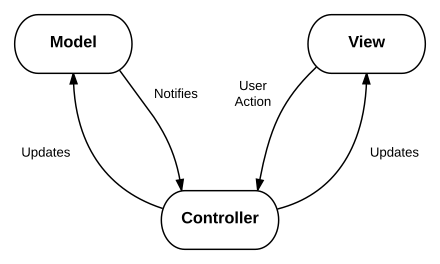
\includegraphics[scale=0.25]{MVC.png}  
\caption{The general structure of the MVC pattern}
\end{figure}    

So the goal is to divide the application in "independent" modules:

\begin{enumerate}

%1, VIEW
\item The view is the surface of the system. In this project it is created with Html, Css, Javascript (with some parts of Php, used to create through the "echo" command part of Html code that are repetitive, for example lists ). The design of the view in this kind of projects is particularly important because the application needs to represent particular kinds of information to particular kinds of users, and both the importance and the special feature needed by this interface are explained in the previous chapters. In the MVC pattern the view is the part less able to "reason" its goal is mainly related to the representation of information. In this project some kind of representations are quite complex, but this complexity is managed by other tiers, and the view needs only to show the users images, html constructions, and 

%2, MODEL
\item In the MVC the model is the central module of the pattern. It contains the application's behavior and must be independent of the user interface. Its primary goal is manage the data of the application. In gAn Web it is a complex situation: excluding some little data related to the configuration and other minor form of persistence, the main data related to this application are the output of another application (gAn). If we consider the whole system the model of the composed application is represented by the the raw root files taken in input by the system. Their loading, interpretation, analysis and activities related to the update of the view are the main activities of the model tier.   

%3, CONTROLLER
\item The main goal of a controller are related to receiving the command of the users, the interpretation of these commands, and the consequent actions to change the state of the model. In gAn Web the controller is represented by the javascript functions able to check, interpret, and send to the server the desires of the users, and the Php scripts able to receive this commands, start the cycle of analysis of the program, and work directly with the model 


\end{enumerate}
 


%the model are root files and root api. the original raw root file? no! this is gAn web not gAn! here the model is the semifnished root files with images and the xml of settings!

%views: html, css (sass to use inheritance), javascript (for client side ad also for interpretation of json), a lot of HCI
%php to generate lists.

%controller: PHPs, able to generate json and able to talk with files and root scripts

\section{Used Technologies}

%sass
%bootstrap
%json

\section{General Schema of the project}

